% #############################################################################
% This is Chapter 2
% !TEX root = ../main.tex
% #############################################################################
% Change the Name of the Chapter i the following line
\fancychapter{Fundamental Concepts}
\cleardoublepage
% The following line allows to ref this chapter
\label{chap:back}

This chapter introduces the fundamental technical concepts and architectures underlying open-vocabulary referring segmentation systems.

% #############################################################################
\section{Neural Networks and Deep Learning}

Neural networks form the foundation of modern deep learning systems, providing the computational framework for learning complex patterns from data. The perceptron represents the simplest form of artificial neural network, consisting of a single computational unit that performs a linear combination of inputs followed by a nonlinear activation function, as illustrated in Figure~\ref{fig:perceptron}. For a perceptron with $N$ input features $\mathbf{x} = [x_1, x_2, \ldots, x_N]^T$, the output $y$ is computed as:

\begin{equation}
y = f(\mathbf{w}^T\mathbf{x} + b),
\end{equation}

where $\mathbf{w} = [w_1, w_2, \ldots, w_N]^T$ represents the weight vector, $b$ is the bias term, and $f(\cdot)$ denotes the activation function. This can be expanded as:

\begin{equation}
y = f\left(\sum_{i=1}^{N} w_i x_i + b\right).
\end{equation}

The activation function $f(\cdot)$ introduces nonlinearity into the model, enabling the perceptron to learn complex decision boundaries. Common activation functions include the sigmoid function $f(z) = \frac{1}{1 + e^{-z}}$, the hyperbolic tangent $f(z) = \tanh(z)$, and the rectified linear unit (ReLU) $f(z) = \max(0, z)$.

Multi-layer perceptrons extend the single perceptron by connecting multiple layers of neurons in a feedforward architecture, as shown in Figure~\ref{fig:mlp}. For a neural network with $L$ layers, where layer $l$ contains $n_l$ neurons, the forward propagation process computes:

\begin{equation}
\mathbf{a}^{(l)} = f^{(l)}\left(\mathbf{W}^{(l)}\mathbf{a}^{(l-1)} + \mathbf{b}^{(l)}\right),
\end{equation}

where $\mathbf{a}^{(l)}$ represents the activation vector of layer $l$, $\mathbf{W}^{(l)} \in \mathbb{R}^{n_l \times n_{l-1}}$ is the weight matrix connecting layers $l-1$ and $l$, $\mathbf{b}^{(l)} \in \mathbb{R}^{n_l}$ is the bias vector, and $f^{(l)}(\cdot)$ is the activation function for layer $l$. The universal approximation theorem demonstrates that multi-layer perceptrons with sufficient hidden units can approximate any continuous function on compact subsets of $\mathbb{R}^n$, providing the theoretical foundation for their expressiveness.

Neural networks are trained through gradient-based optimization methods that minimize a loss function $\mathcal{L}(\theta)$, where $\theta$ represents all learnable parameters. The loss function quantifies the difference between predicted outputs and ground truth targets, such as the mean squared error for regression tasks:

\begin{equation}
\mathcal{L}(\theta) = \frac{1}{n}\sum_{i=1}^{n}(y_i - \hat{y}_i)^2,
\end{equation}

where $n$ is the number of training samples, $y_i$ are the true labels, and $\hat{y}_i$ are the predicted outputs. The backpropagation algorithm efficiently computes gradients by applying the chain rule of calculus. The most common optimization algorithm is stochastic gradient descent, which updates parameters according to:

\begin{equation}
\theta_{t+1} = \theta_t - \eta \nabla_\theta \mathcal{L}(\theta_t),
\end{equation}

where $\eta$ is the learning rate and $\nabla_\theta \mathcal{L}(\theta_t)$ represents the gradient of the loss function with respect to parameters at iteration $t$.

\begin{figure}[t]
\centering
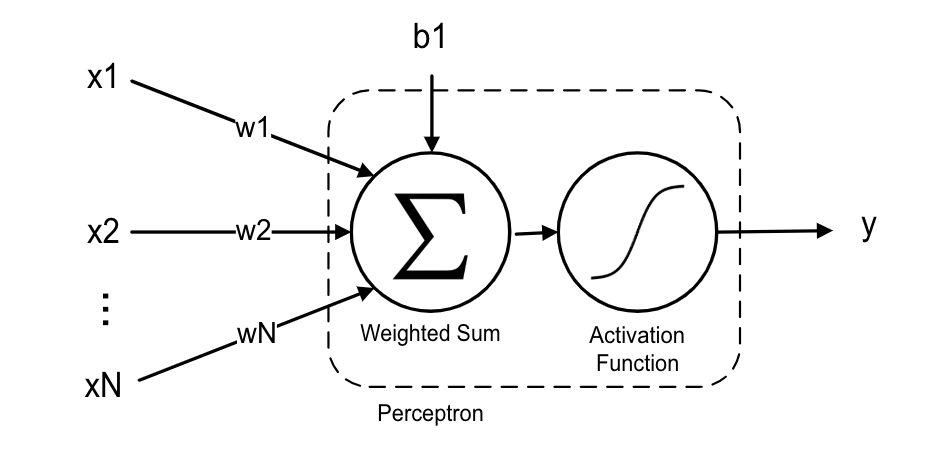
\includegraphics[width=0.6\textwidth]{Images/perceptron.png}
\caption{Perceptron architecture and basic neural network building block.}
\label{fig:perceptron}
\end{figure}

\begin{figure}[htbp]
\centering
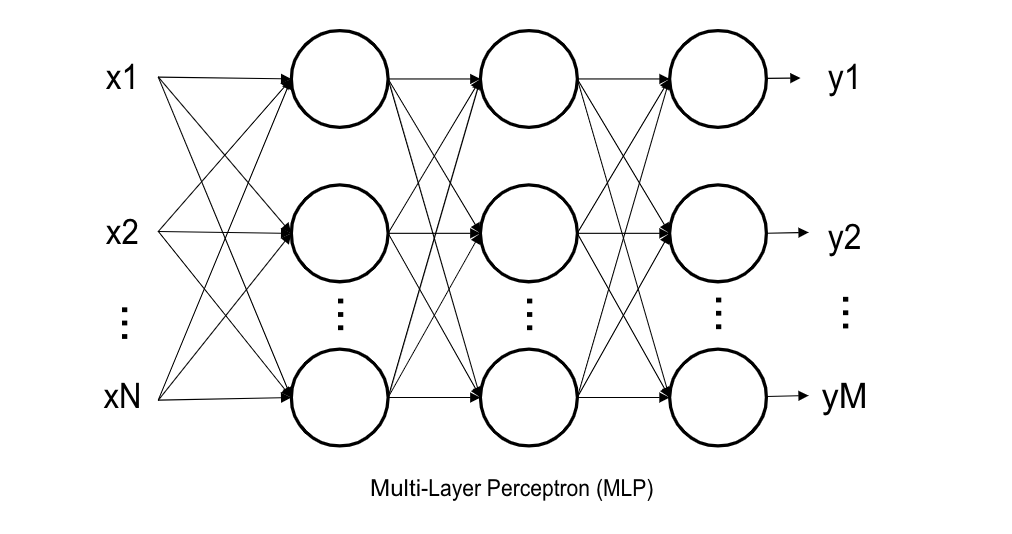
\includegraphics[width=0.6\textwidth]{Images/mlp.png}
\caption{Multi-layer perceptron architecture showing feedforward neural network structure.}
\label{fig:mlp}
\end{figure}

% #############################################################################
\section{Attention and Transformers}

The transformer architecture revolutionized sequence modeling by introducing a self-attention mechanism that enables models to process variable-length sequences more effectively than traditional fixed-size approaches. Unlike multi-layer perceptrons that operate on fixed-dimensional inputs, transformers can handle sequences of arbitrary length and are particularly effective at capturing long-range dependencies in medium to long sequences through the self-attention mechanism, making them suitable for tasks across multiple modalities including natural language, vision, audio, time series, or any sequential data where relationships between distant elements are important.

The core innovation of transformers lies in the self-attention mechanism, which allows each element in a sequence to attend to all other elements simultaneously, as illustrated in Figure~\ref{fig:transformer}. For a sequence of input tokens represented as embeddings $\mathbf{X} = [\mathbf{x}_1, \mathbf{x}_2, \ldots, \mathbf{x}_n] \in \mathbb{R}^{n \times d}$, where $n$ is the sequence length and $d$ is the embedding dimension, the self-attention mechanism computes three matrices: queries ($\mathbf{Q}$), keys ($\mathbf{K}$), and values ($\mathbf{V}$):

\begin{equation}
\mathbf{Q} = \mathbf{X}\mathbf{W}_Q, \quad \mathbf{K} = \mathbf{X}\mathbf{W}_K, \quad \mathbf{V} = \mathbf{X}\mathbf{W}_V,
\end{equation}

where $\mathbf{W}_Q, \mathbf{W}_K, \mathbf{W}_V \in \mathbb{R}^{d \times d_k}$ are learned parameter matrices. The attention scores $\boldsymbol{\alpha}$ are computed as:

\begin{equation}
\boldsymbol{\alpha} = \text{softmax}\left(\frac{\mathbf{Q}\mathbf{K}^T}{\sqrt{d_k}}\right),
\end{equation}

where the scaling factor $\sqrt{d_k}$ prevents the softmax function from saturating for large embedding dimensions. The final attention output is then computed as:

\begin{equation}
\text{Attention}(\mathbf{Q}, \mathbf{K}, \mathbf{V}) = \boldsymbol{\alpha}\mathbf{V},
\end{equation}

where $\boldsymbol{\alpha}$ represents the attention weights that determine how much each value $\mathbf{V}$ contributes to the output.

Since transformers process all positions in parallel, they lack inherent positional information. To address this, positional encodings are added to input embeddings to provide the model with information about token positions. The original transformer uses sinusoidal positional encodings:

\begin{equation}
PE_{(pos, 2i)} = \sin\left(\frac{pos}{10000^{2i/d}}\right), \quad PE_{(pos, 2i+1)} = \cos\left(\frac{pos}{10000^{2i/d}}\right),
\end{equation}

where $pos$ is the position index and $i$ is the dimension index. This encoding scheme allows the model to learn relative positions and generalizes to sequences longer than those seen during training.

The transformer block combines self-attention with feed-forward layers and residual connections. Each block applies layer normalization before both the attention and feed-forward operations, following the pre-normalization variant. The complete transformation for a single transformer block can be expressed as:

\begin{equation}
\mathbf{H}' = \text{Attention}(\text{LayerNorm}(\mathbf{H})) + \mathbf{H},
\end{equation}

\begin{equation}
\mathbf{H}'' = \text{FFN}(\text{LayerNorm}(\mathbf{H}')) + \mathbf{H}',
\end{equation}

where $\mathbf{H}$ represents the input hidden states and FFN denotes the feed-forward network. Multiple transformer blocks can be stacked to create deeper models that capture increasingly complex patterns in the input sequences.

\begin{figure}[tb]
\centering
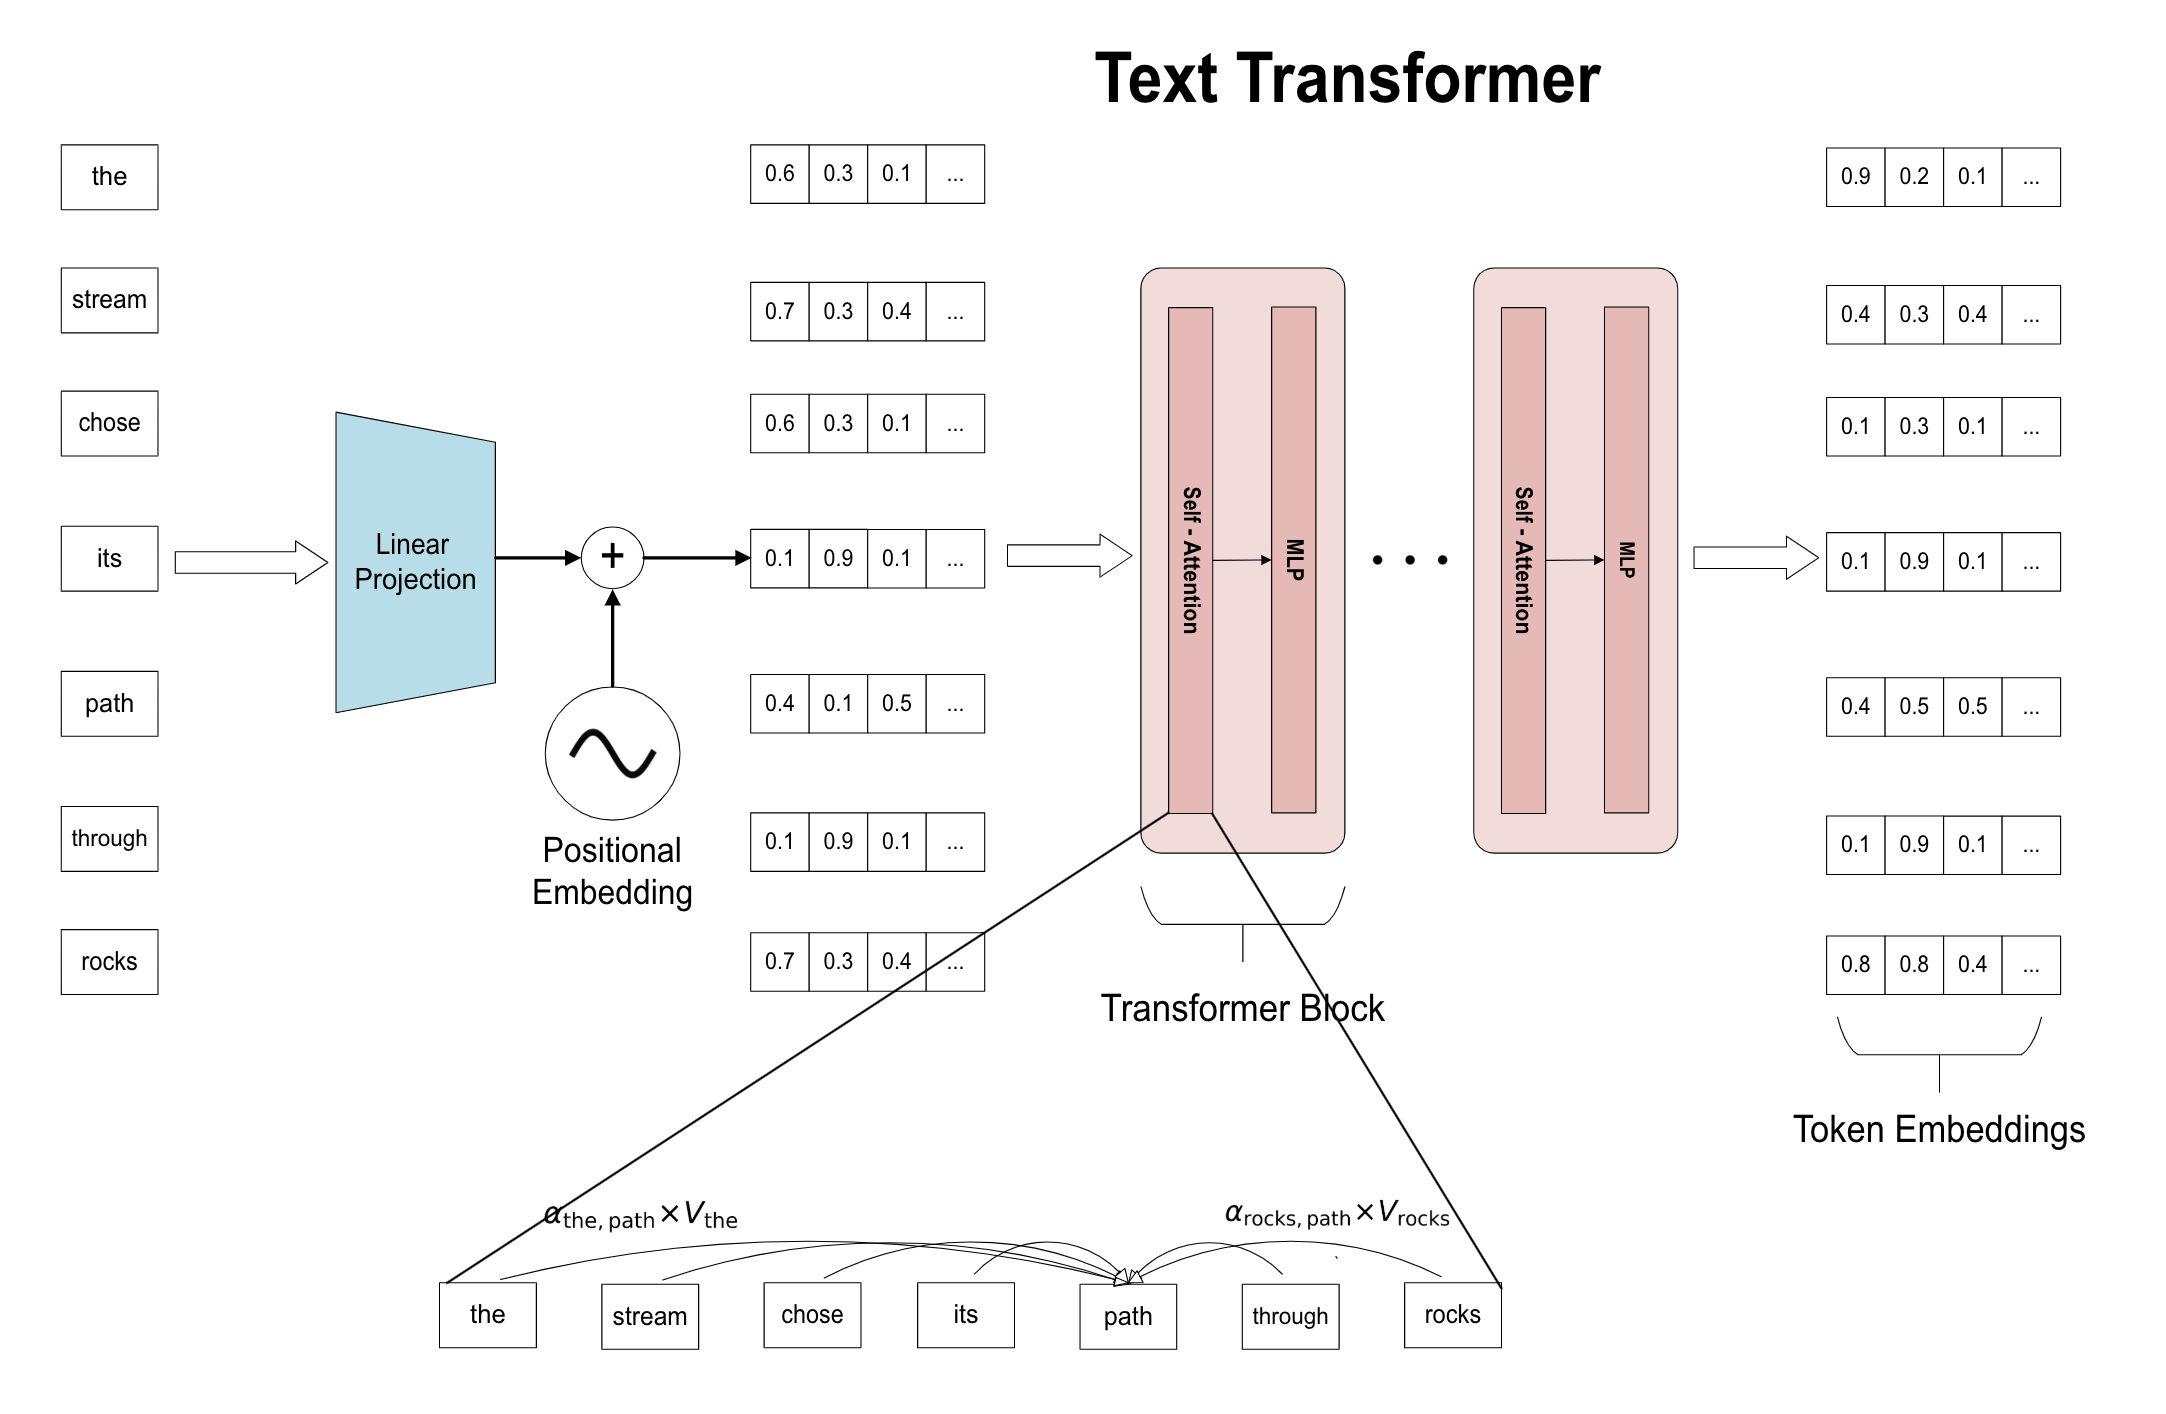
\includegraphics[width=0.9\textwidth]{Images/transformer.png}
\caption{Self-attention mechanism in transformers. The diagram shows how attention scores $\alpha$ are computed for each token, with specific examples of attention weights for tokens "path" and "rocks" relative to other words in the sequence "the stream chose its path through rocks".}
\label{fig:transformer}
\end{figure}

% #############################################################################
\section{Transformers for Computer Vision}

Application of transformer architectures to computer vision tasks and visual understanding.

\begin{figure}[htbp]
\centering
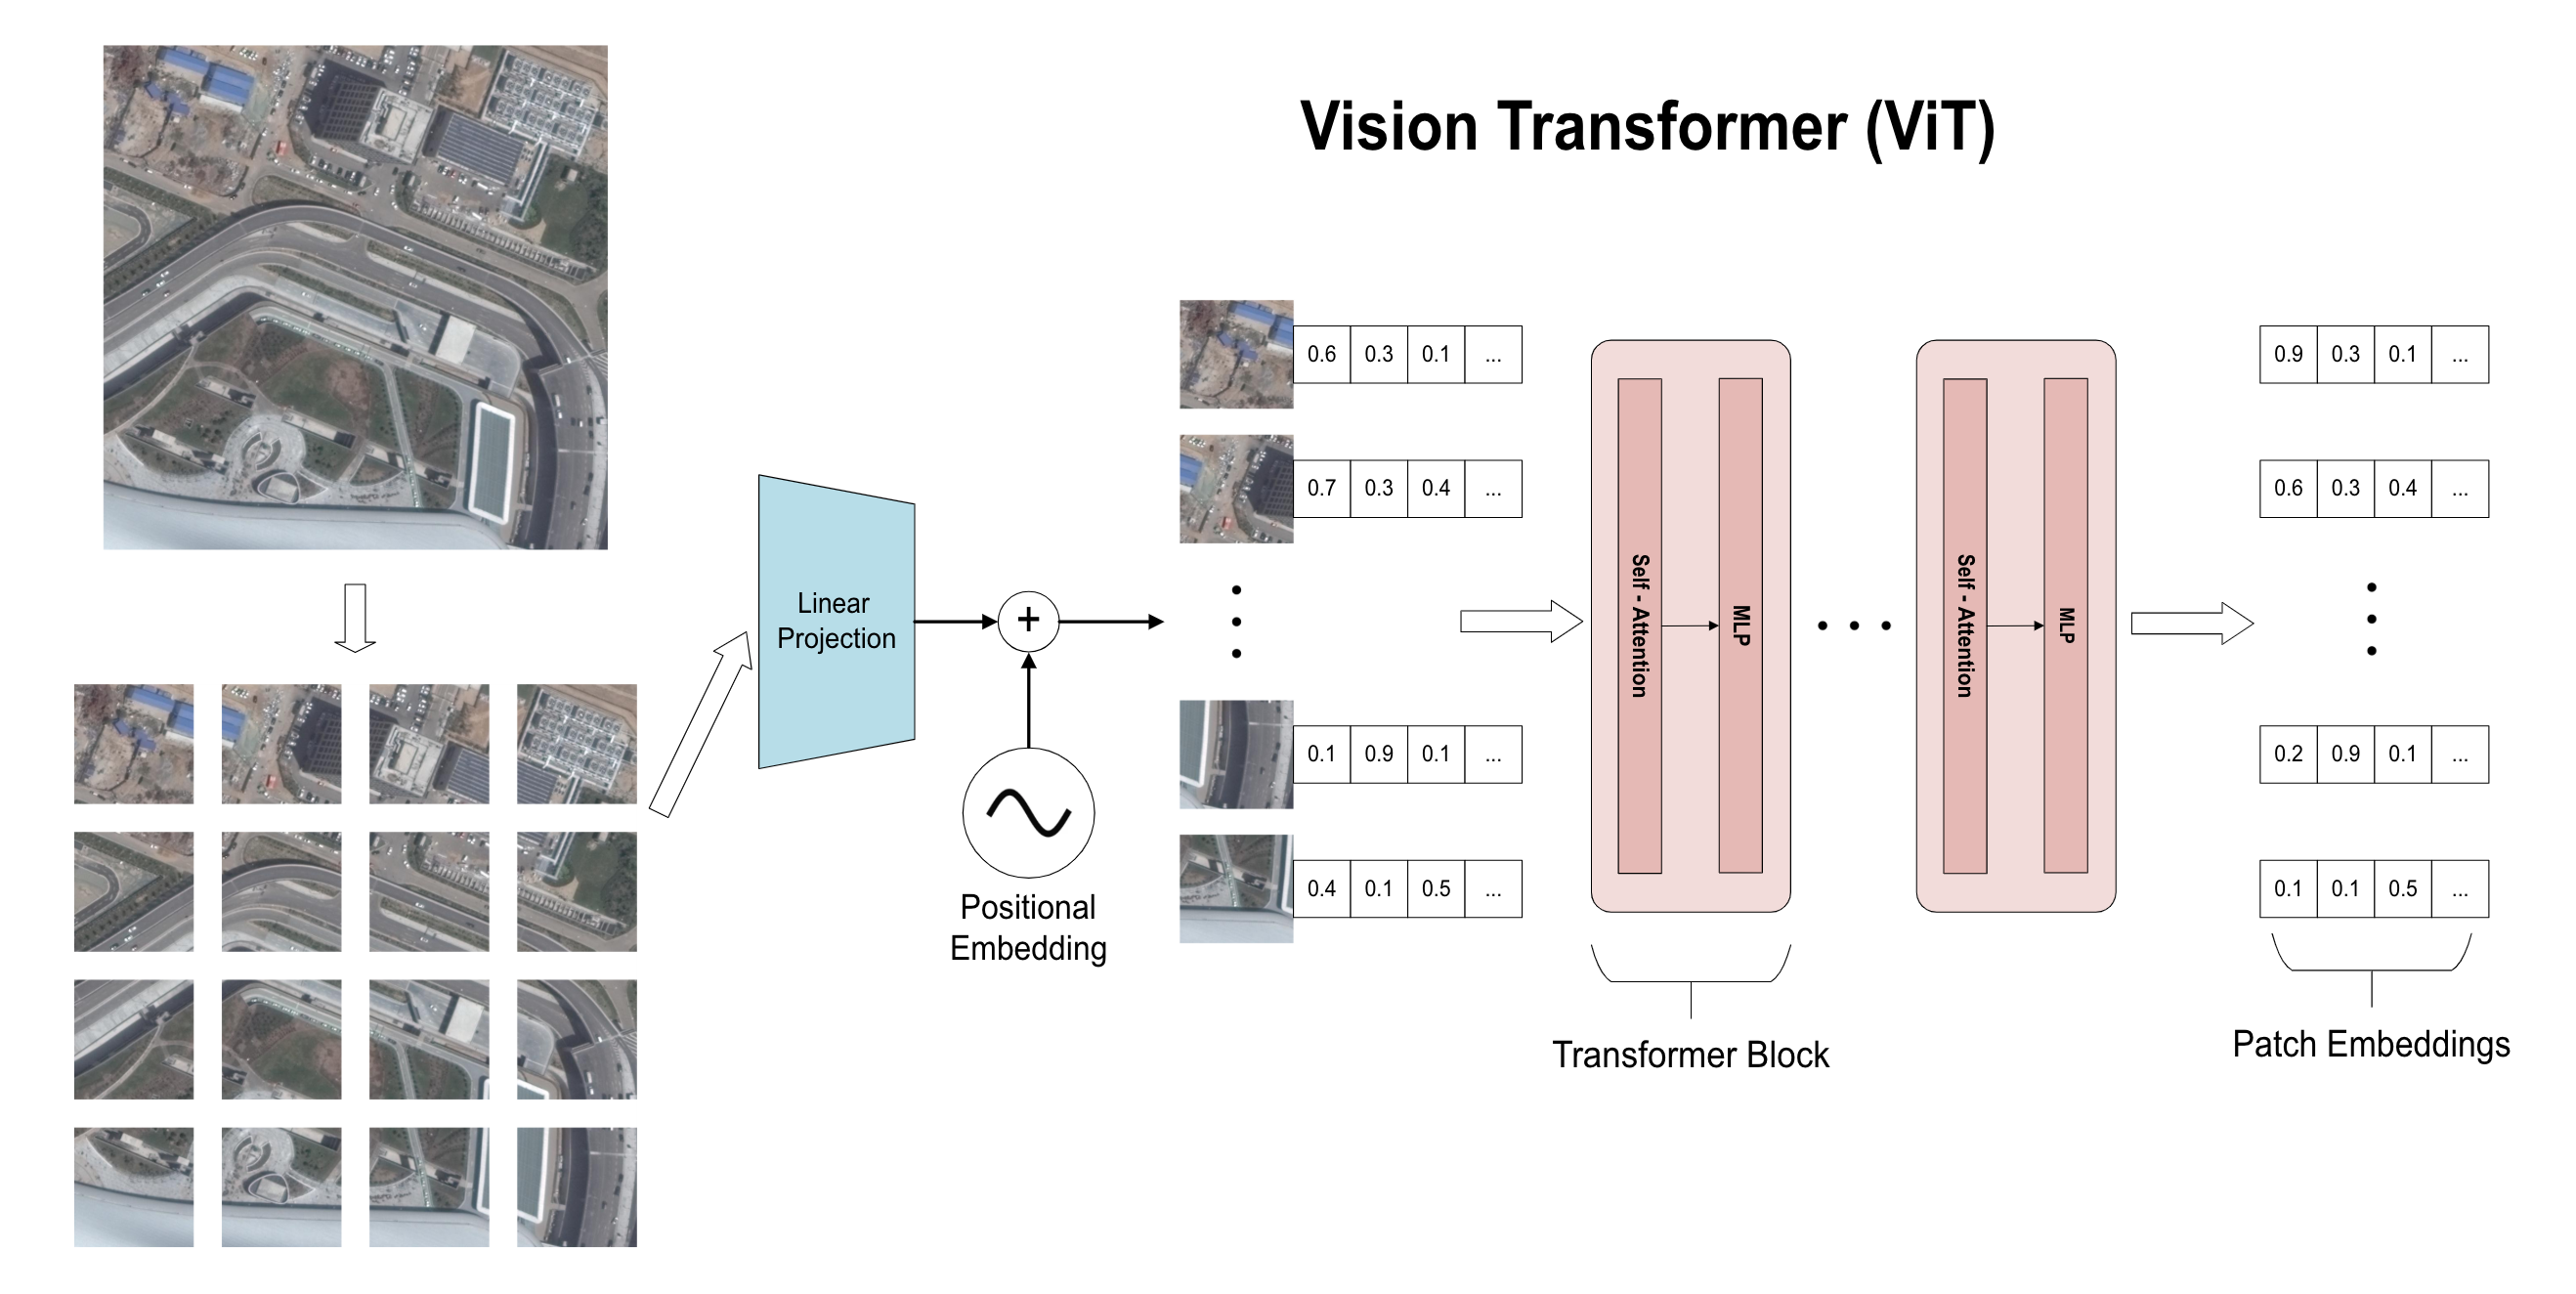
\includegraphics[width=0.8\textwidth]{Images/vit.png}
\caption{Vision Transformer (ViT) architecture for image classification and feature extraction.}
\label{fig:vit}
\end{figure}

% #############################################################################
\section{Image Segmentation}

Deep learning approaches for image segmentation tasks and methodologies.

\begin{figure}[htbp]
\centering
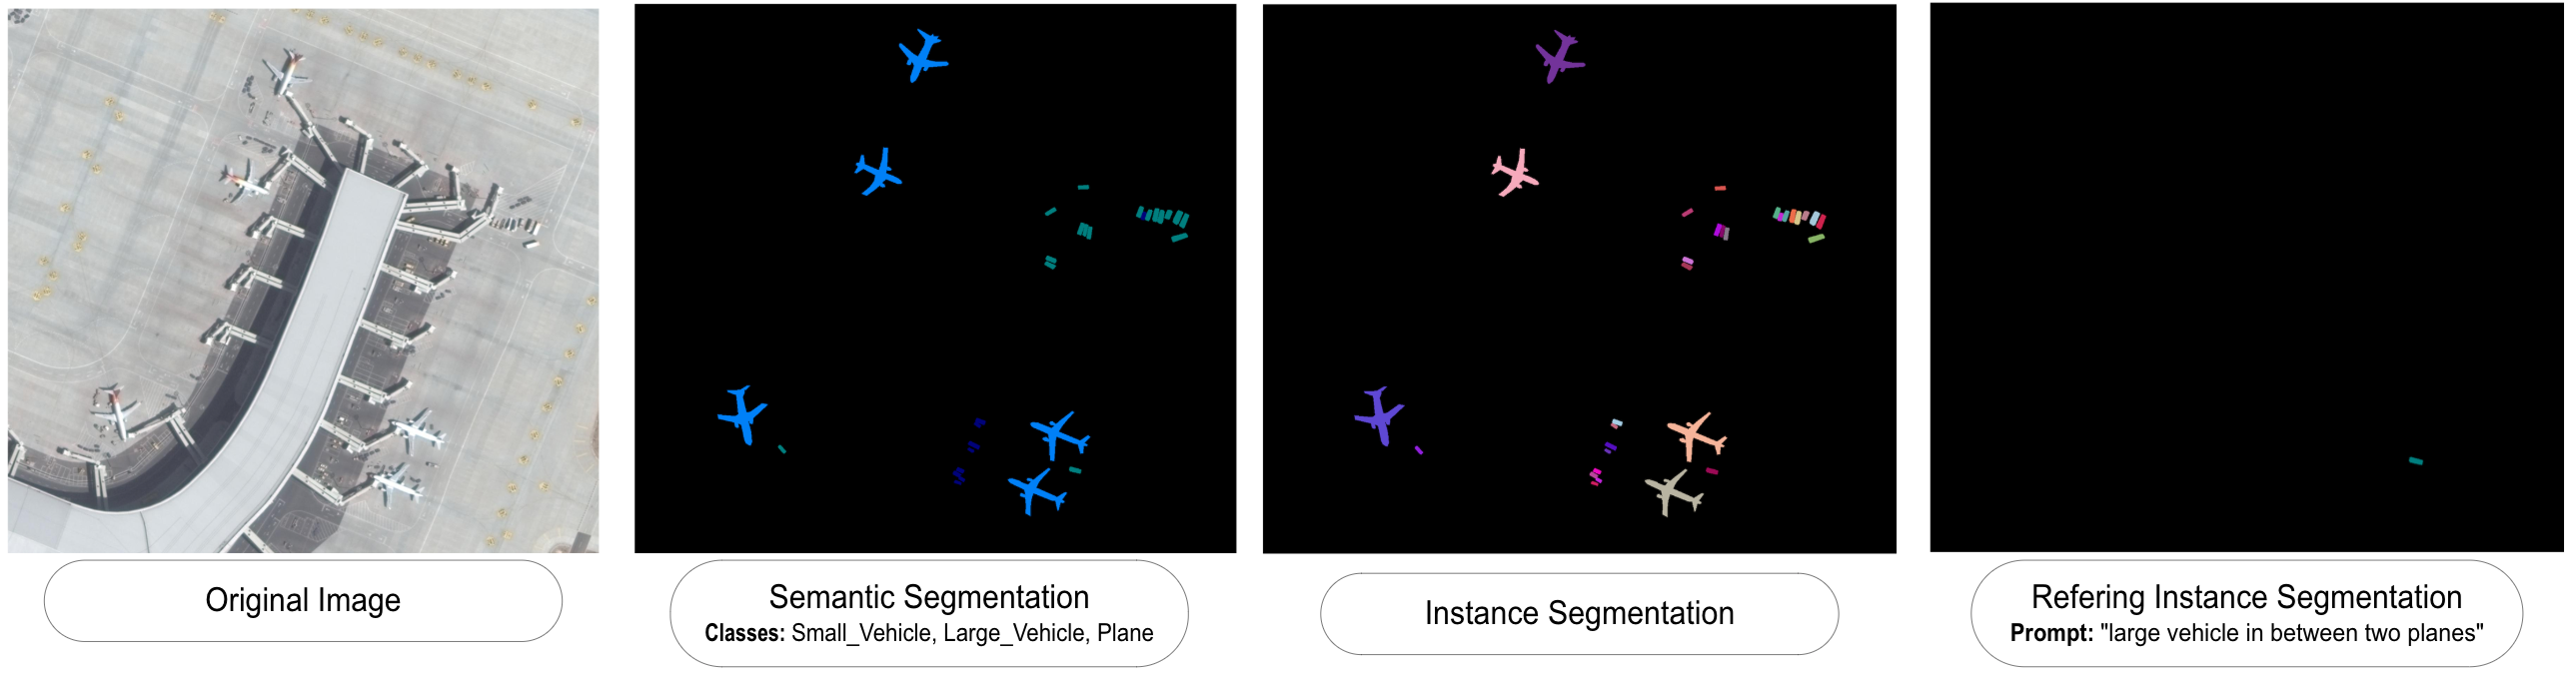
\includegraphics[width=1.0\textwidth]{Images/segmentation.png}
\caption{Comparison of segmentation types: semantic segmentation, instance segmentation, and referring instance segmentation with natural language prompts.}
\label{fig:segmentation}
\end{figure}

% #############################################################################
\section{Vision-Language Models}

Multimodal architectures that process both visual and textual information.

\subsection{CLIP and Visual-Language Learning}

Contrastive Language-Image Pre-training model architecture and visual-language learning methodologies.

\begin{figure}[htbp]
\centering
\subfigure[Contrastive pre-training methodology.]{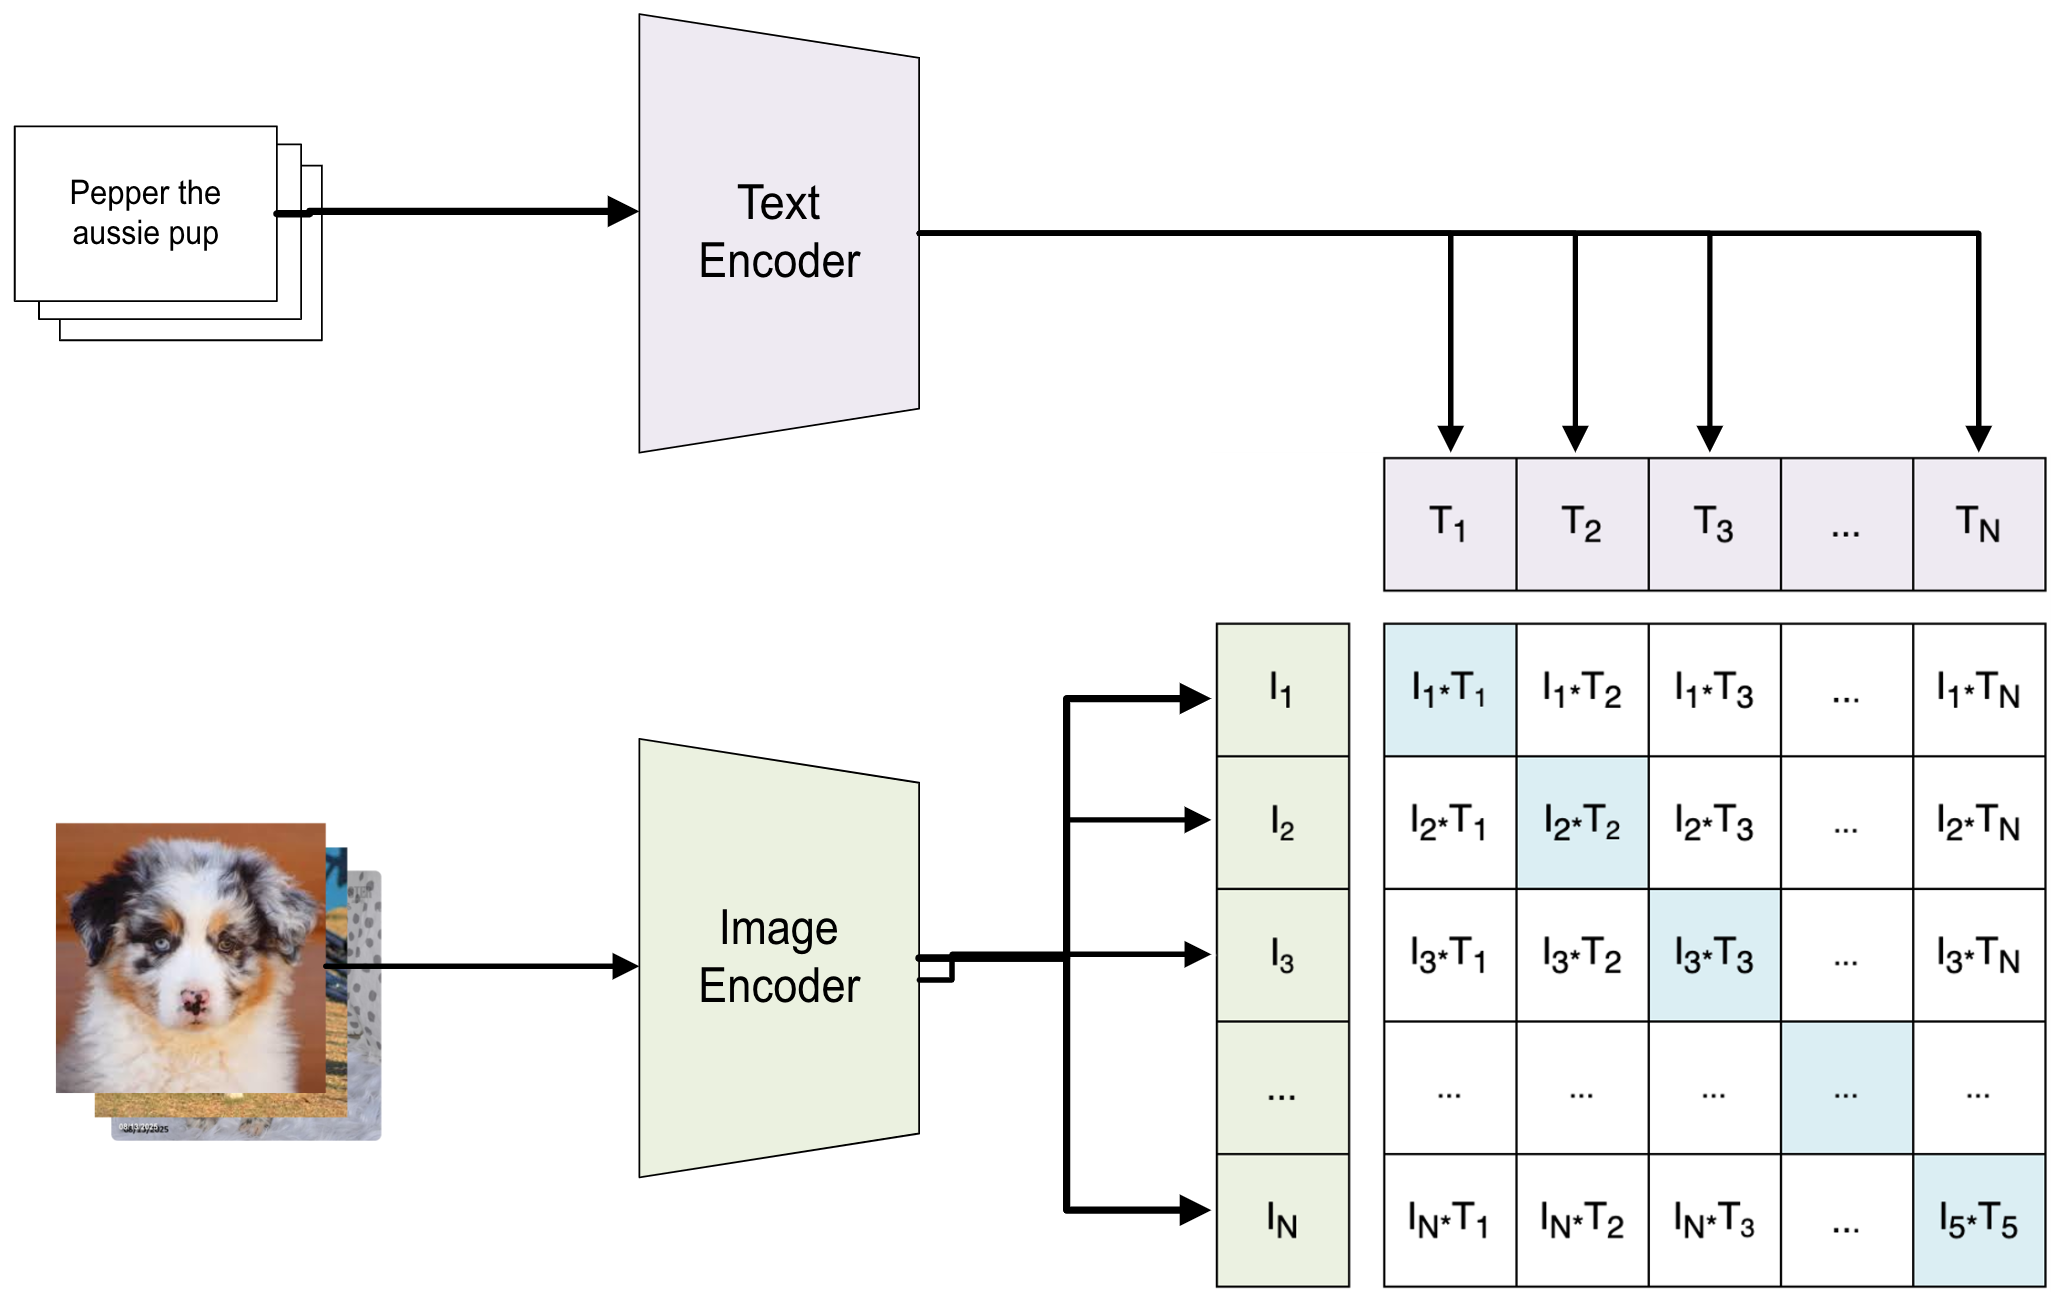
\includegraphics[width=0.45\textwidth]{Images/contrastive_pretraining.png}\label{fig:contrastive_pretraining}}
\hfill
\subfigure[Zero-shot prediction capabilities.]{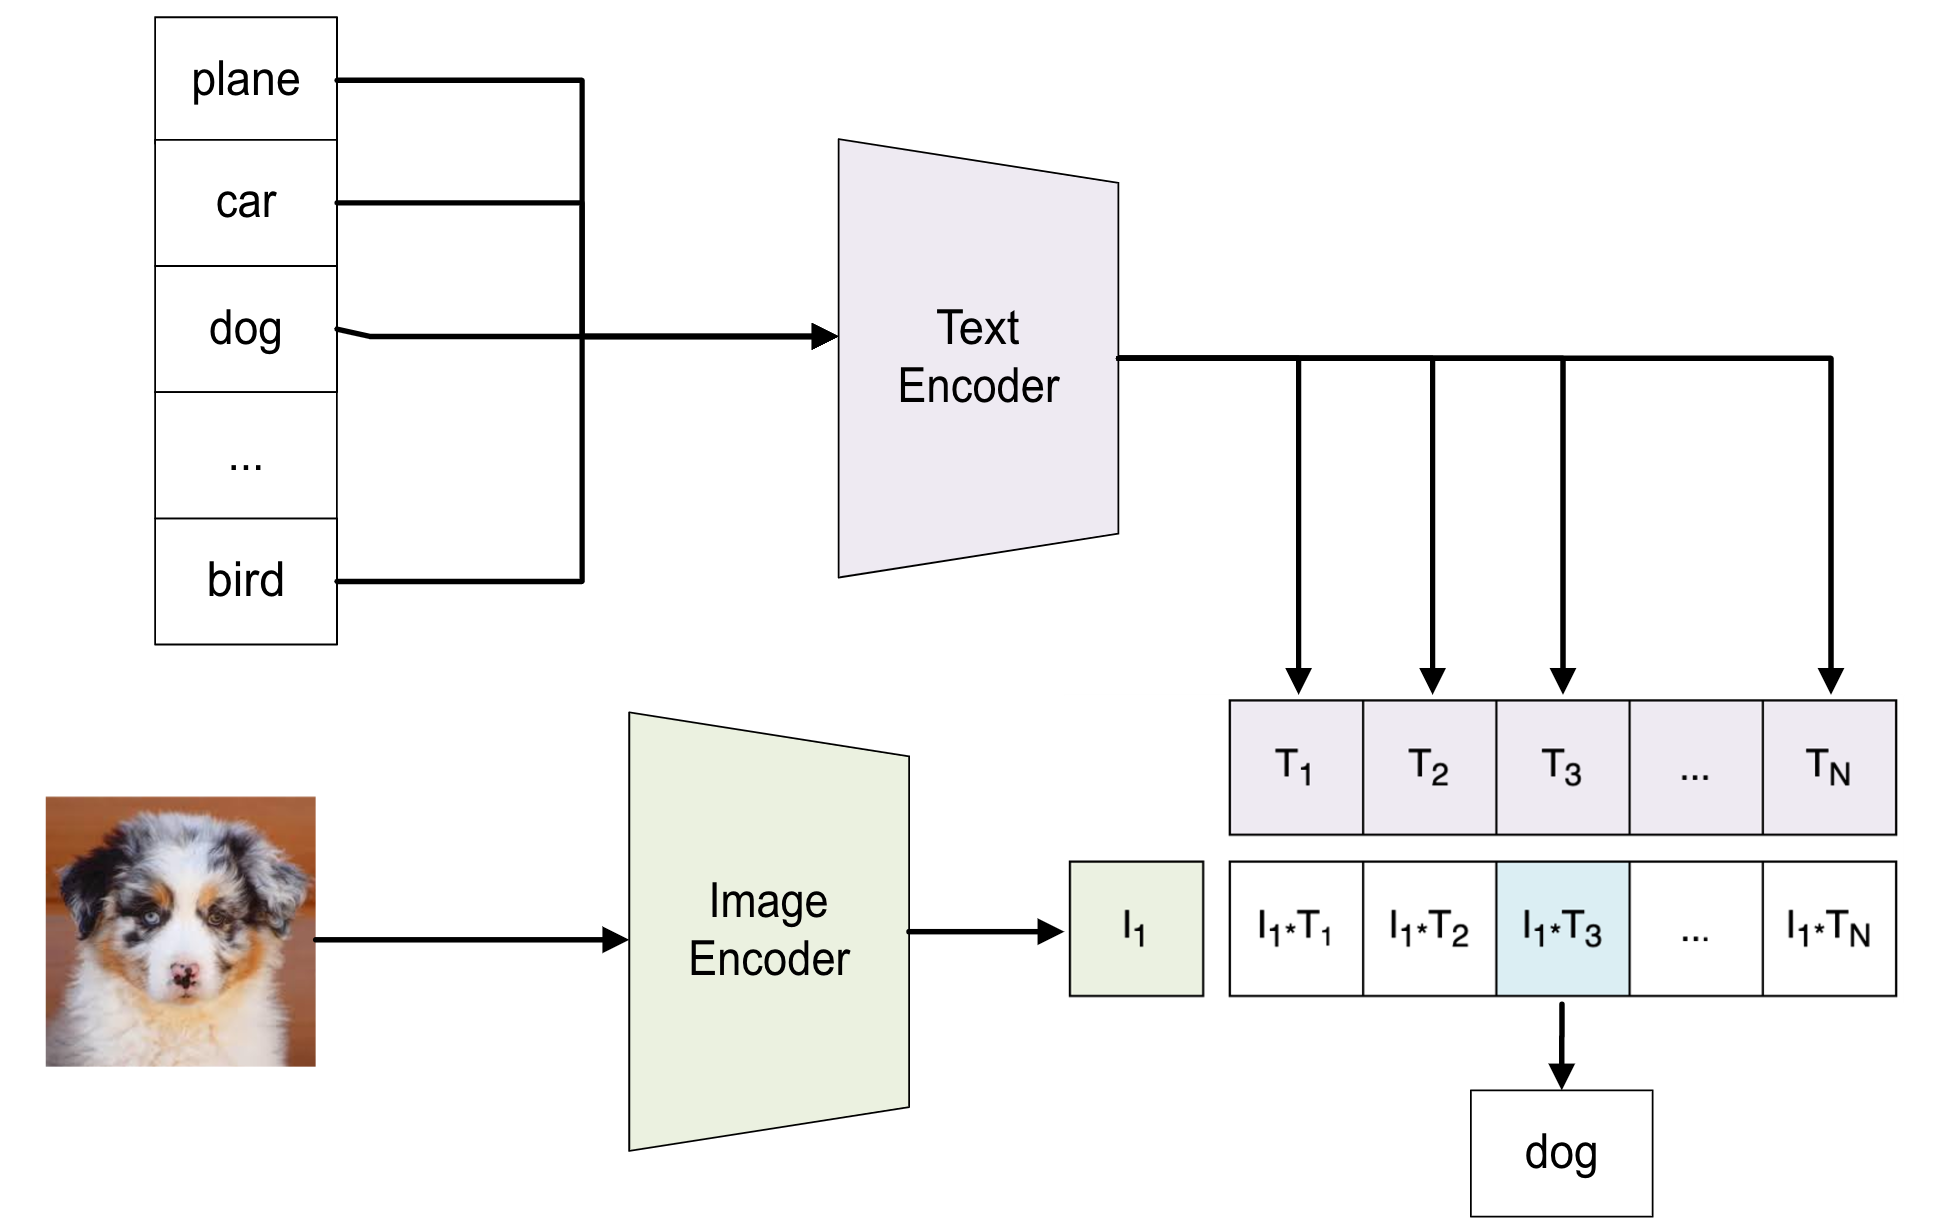
\includegraphics[width=0.45\textwidth]{Images/zero_shot_prediction.png}\label{fig:zero_shot_prediction}}
\caption{CLIP architecture components showing contrastive pre-training and zero-shot prediction mechanisms.}
\label{fig:clip_architecture}
\end{figure}

\subsection{Large Language Models}

Foundation models for natural language understanding and generation in multimodal contexts.

\begin{figure}[htbp]
\centering
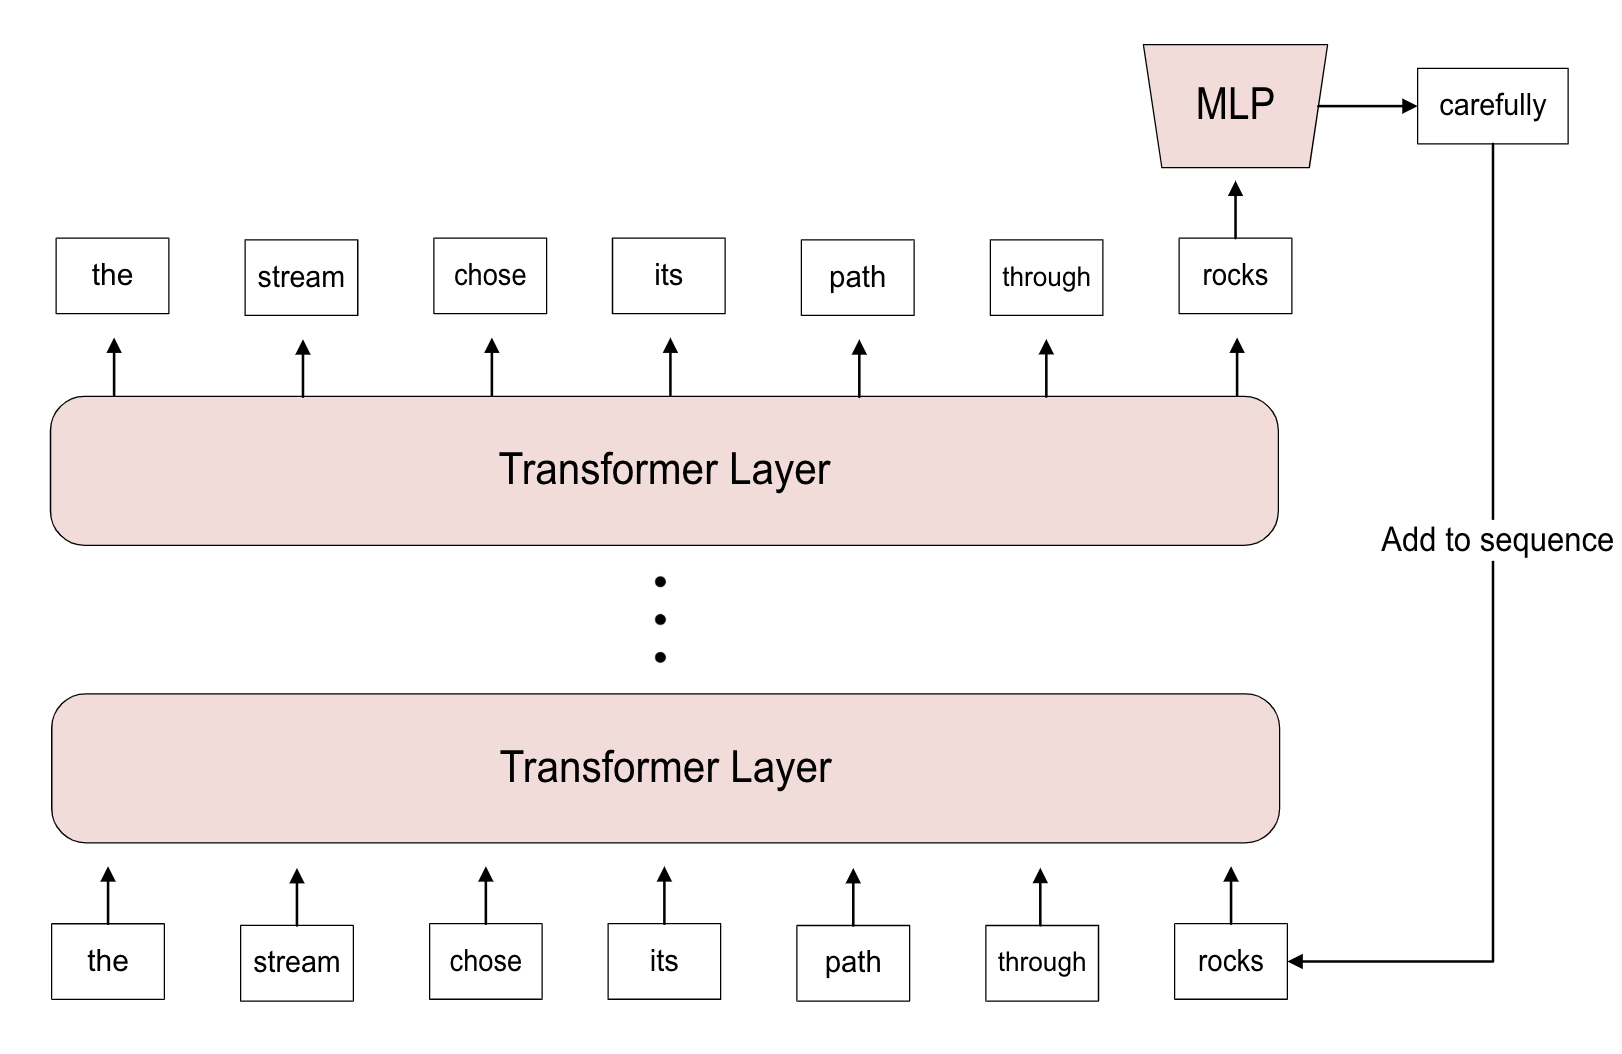
\includegraphics[width=0.8\textwidth]{Images/gpt.png}
\caption{GPT autoregressive language model architecture showing the transformer decoder stack with next-token prediction and feedback mechanism.}
\label{fig:gpt}
\end{figure}